\newpage
\section{Durchführung}
In diesem Teil wird die Durchführung des Versuchs beschrieben.

\subsection{Prinzipielle Funktionsweise}
Zunächste wird der prinzipielle Aufbau eines Lock-In Verstärkers auf zwei Arten untersucht. Zum einen durch ein Nutzsignal welches von einem Sinusgenerator kommt und einmal ein Nutzsignal welches Störungen besitzt. Der schematische Aufbau der Apperatur ist in der \autoref{fig:2} dargestellt. Bei beiden Signalen ist das Vorgehen der Untersuchung identisch.

\begin{figure}[H]
    \centering
    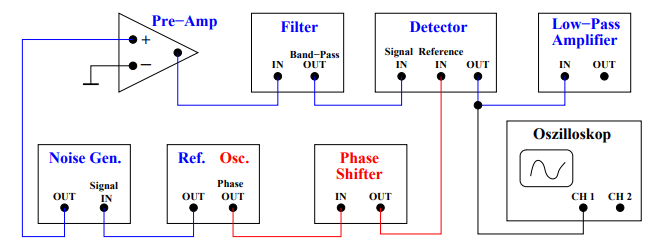
\includegraphics{Picture/2.png}
    \caption{Schematischer Aufbau des Versuches \cite{V303}}
    \label{fig:2}
\end{figure}

\noindent
Zur Untersuchung wird ein Oszilloskop an den Mischer angeschlossen und das Mischsignal wird betrachtet. Dazu wird das Mischsignal bei mindestens 10 verschiedenen Phasendifferenzen aufgenommen und auf einem Stick gespeichert.

\newpage
\subsection{LED - Photodiode}
Zusätzlich zur normalen Untersuchung des Mischsignals wird über eine Photodetektorschaltung das Signal der Photodiode in Abhängigkeit des Abstands zwischen LED und Photodiode untersucht. Der neue Aufbau ist in der \autoref{fig:3} abgebildet.

\begin{figure}[H]
    \centering
    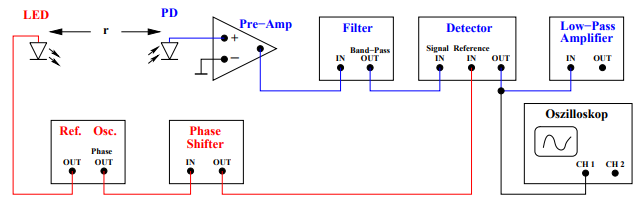
\includegraphics{Picture/3.png}
    \caption{Aufbau der Photodetektorschaltung \cite{V303}}
    \label{fig:3}
\end{figure}
\noindent